\documentclass[11pt,a4paper]{article}

% Packages
\usepackage{geometry}
\usepackage{setspace}
\usepackage{graphicx}
\usepackage{lipsum}
\usepackage{url}
\usepackage{hyperref}
\hypersetup{
    colorlinks=true,
    linkcolor=blue, % or cyan
    urlcolor=blue, % or cyan
    citecolor=blue, % or cyan
}
\usepackage{csquotes}
\usepackage{xcolor}
\usepackage{booktabs}
\usepackage{listings}
\usepackage{subcaption} % Add this line to import the subcaption package
\usepackage{wasysym}
\usepackage{seqsplit}




\definecolor{codegreen}{rgb}{0,0.6,0}
\definecolor{codegray}{rgb}{0.5,0.5,0.5}
\definecolor{codepurple}{rgb}{0.58,0,0.82}
\definecolor{backcolour}{rgb}{0.95,0.95,0.92}

\lstdefinestyle{mystyle}{
    backgroundcolor=\color{backcolour},   
    commentstyle=\color{codegreen},
    keywordstyle=\color{magenta},
    numberstyle=\tiny\color{codegray},
    stringstyle=\color{codepurple},
    basicstyle=\ttfamily\footnotesize,
    breakatwhitespace=false,         
    breaklines=true,                 
    captionpos=b,                    
    keepspaces=true,                 
    numbers=left,                    
    numbersep=5pt,                  
    showspaces=false,                
    showstringspaces=false,
    showtabs=false,                  
    tabsize=2
}

\lstset{style=mystyle}


% Page formatting
\geometry{a4paper, margin=1in}
\renewcommand{\baselinestretch}{1.0}
\setlength{\parskip}{1em}
\pagenumbering{arabic}

% Bibliography
\usepackage[
    backend=biber,
    style=nature
]{biblatex}
\addbibresource{references.bib}

\begin{document}

% % Title
% \title{AI-assisted Design of virus-binding proteins for the International Genetically Engineered Machine comptetion}
% \author{Tony MAKDISSY\thanks{Learning Planet Institute}}




% \date{August 2023 -- November 2023}
% \maketitle

\begin{titlepage}
    \centering
    
    {\scshape\Large Learning Planet Institute \par}
    % \vspace{1cm}
    {\scshape\Large Université Paris Cité \par}
    \vspace{0.5cm}
    {\scshape\Large Master AIRE Life Sciences \par}

    \begin{minipage}{0.25\textwidth}
        
\includegraphics[width=\linewidth]{Logos/UniversiteParisCite_logo_horizontal_couleur_RVB_Couleur.png}\par\vspace{1cm}
        
\includegraphics[width=\linewidth]{Logos/PIA_logo.png}\par\vspace{1cm}
    \end{minipage}
    \begin{minipage}{0.25\textwidth}
        % project_logo.png
        
\includegraphics[width=\linewidth]{Logos/project_logo.png}\par\vspace{1cm}
        
\includegraphics[width=\linewidth]{Logos/Copie de LPI_LOGO_RVB.png}\par\vspace{1cm}
    \end{minipage}
    \begin{minipage}{0.25\textwidth}
        
\includegraphics[width=\linewidth]{Logos/EURIP logo.png}\par\vspace{1cm}
        
\includegraphics[width=\linewidth]{Logos/SmartUP_1920-1 (1).png}\par\vspace{1cm}
    \end{minipage}

    {\scshape\Large AI-assisted Design of virus-binding proteins for the International
    Genetically Engineered Machine competition iGEM \par}
    \vspace{1cm}

    {\huge\bfseries Tony MAKDISSY \par}
    \vspace{1cm}

    \textbf{Team Members:}
    
    Milena MILOVANOVIC, Avishkar JADHAV, Louis ELVERSTON, Mostafa ELRAIES, Joann LEVAY, Laure Mourgue D'ALGUE, Dakshayani PINNINTI, Stasa RAKOCEVIC, \\ and Hritika KATHURIA
    \vspace{0.5cm}
    
    \textbf{Supervisors:}

    Ariel LINDNER, Ernest MORDRET, Helena SHOMAR, and Amir PANDI

    \vfill

    % Bottom of the page
    {\large July 2023 - November 2023\par}
\end{titlepage}

\tableofcontents
\newpage

% Abstract
\begin{abstract}

    The field of \emph{de novo} protein design has witnessed significant advancements, evolving from manual crafting to sophisticated computational methodologies. This report details an exploration into de novo protein design, specifically focusing on the computational pipeline developed for generating potential protein binders. Leveraging tools like RFdiffusion, HDOCK, and ChimeraX. A theoretically automated workflow was employed to inspect target proteins, identify hotspots, and validate sequences through pull-down assays. Despite challenges in automating hotspot identification and GPU-dependent execution, the pipeline demonstrated promising results. Three sequences exhibited positive binding to the T4 bacteriophage, showcasing the feasibility of this approach. The success of this proof-of-concept provides a foundation for scaling up the design and exploring more complex protein structures.
    
\end{abstract}

% General Context
\section{General Context}

% What is iGEM
This report details my involvement in the Paris-Bettencourt team's 
collaborative participation in the International Genetically Engineered 
Machine (iGEM) contest \cite{igem_main}. The iGEM competition, held annually, 
is a globally recognized Synthetic Biology competition, uniting 
participants across three distinct age groups: high school, 
undergraduate, and graduate students from all over the world
\cite{igem_description}.
% villages
The topics covered by the competition are divided into 15 themes called villages \cite{igem_villages}.
Paris-Bettencourt project, named "Lubritect", was part of the Therapeutics village.

% Lubritect project
Lubritect is designed to be an innovative solution that combines 
mucin-based hydrogel with AI-generated protein structures, aiming to 
reduce the transmission of sexually transmitted infections (STIs). This 
approach leverages \emph{de novo} protein design for versatility against 
various pathogens. 
Lubritect targeted 5
sustainable development goals:
\begin{itemize}
    \item SDG3 (Good health and wellbeing)
    \item SDG4 (Inclusive and equitable quality education and promote lifelong learning opportunities for all)
    \item SDG5 (Achieve gender equality and empower all women and girls)
    \item SDG8 (Decent Work and Economic Growth)
    \item SDG12 (Responsible Consumption and Production)
\end{itemize}

All while trying to follow the Free and Open-Source Software (FOSS) philosophy \cite{gun_foss} by using free and open-source tools and making sure that all our codes and results are available via the iGEM website.

% Team composition
Paris-Bettencourt team is hosted by Learning Planet Institute (LPI),
consisting of 7 LPI students, and 3 Non-LPI students.
Each has a specific role like wet-lab, dry-lab, or human practices \ldots etc. With 4 supervisors who oversaw the project and offered scientific and emotional help \cite{paris_bettencourt_team}.
% My role
My main role in this project was generating and \emph{in-silico} testing of new protein structures to bind to the targets of interest.


% Introduction
\section{Introduction}

\emph{de novo} Protein design is the field of science that addresses the 
fundamental question: "Is our knowledge of the principles of folding 
and function sufficient to design proteins from scratch?" 
\cite{korendovych2020novo} or, in broader terms, "Are natural proteins 
special? Can we do that?" \cite{hecht2018natural}.

\subsection{History of \emph{de novo} protein design}

According to Korendovych and DeGrado \cite{korendovych2020novo}, \emph{de novo} 
protein design has evolved through several stages.
In the nascent days of \emph{de novo} protein design, researchers manually 
crafted protein structures. A landmark achievement occurred in 1983 
when Moser et al. successfully designed a DDT binder through manual 
intervention \cite{moser1983artificial}.
The field transitioned towards computational approaches, where proteins 
are designed using computers and guided by physicochemical principles 
of protein folding. One notable example is the protein designed by 
DeGrado, Regan, and Ho in 1987 \cite{degrado1987design}. In this 
groundbreaking work, the team successfully crafted a 4-helix 
homo-multimer, with each helix comprising 16 residues. The helices were 
strategically composed, featuring Leucine for hydrophobicity in the 
inner lumen of the helix, and Glutamic acid and Lysine for the external 
region of the helix. Additionally, Glycine was employed to disrupt the 
helix. This meticulous design strategy significantly reduced the 
potential residues' composition from $20^{16}$ (approximately 6.5 * $10^
{20}$) possibilities to fewer than a thousand, thereby narrowing the 
design space significantly. 
Later on, in the early 2000s, with the accumulation of a vast repository 
of crystallized protein structures,  marked the advent of 
fragment-based and bioinformatics-informed methods. Notably, this era 
saw the design of a  TOP7 protein, incorporating fragments from the 
Protein Data Bank to construct a structure not observed in nature \cite
{kuhlman2003design}.

\subsection{Advancements in Molecular and Computational Biology}

The advent of accurate protein structure prediction tools exemplified 
by AlphaFold2 \cite{jumper2021highly}, RoseTTAFold \cite
{baek2021accurate}, and ESMFold \cite{lin2022language}, significantly 
impacted \emph{de novo} protein design. These tools facilitated in-silico 
testing of designed protein structures, reducing the need for extensive 
experimental validation and enabling exploration beyond natural 
sequences.
Along with the advancements in computational capabilities, DNA synthesis 
and high-throughput screening methods have accelerated \emph{de novo} protein 
design. Recent achievements include the creation of mechanically 
coupled  axle-rotor proteins by a team from the Baker lab, University 
of Washington \cite{courbet2022computational,bakerlab}, where the team 
discovered a wide variety of designs aided by computational simulations.

\subsection{Machine Learning in \emph{de novo} protein design}

Despite these advancements, the field is limited by the vast number of 
possible protein structures. Machine learning (ML) approaches 
aim to overcome this challenge by training models to design proteins 
with specific structures or functions. Message Passing Neural Networks 
(MPNNs), exemplified by ProteinMPNN \cite{dauparas2022robust} developed 
by Baker lab, play a  crucial role in predicting amino acid sequences 
starting from a given structure.
In March 2023 Baker Lab published RFdiffusion, a successor of 
ProteinMPNN, which is a diffusion model trained on protein sequences and 
structures from Protein Data Bank (PDB) with structures generated by 
RoseTTAFold and AlphaFold2. RFdiffusion stands out as an innovative 
tool for \emph{de novo} protein design. It allows for the generation of new 
protein sequences based on specified constraints such as sequence 
length, binding properties, and amino acid sequences \cite{
watson2023novo}. It does so by first predicting a suitable structure 
for the given constraints, then generating a sequence that folds into 
the predicted structure using ProteinMPNNs.
The field of \emph{de novo} protein design also welcomed other ML approaches, 
such as RosettaSurf \cite{scheck2022rosettasurf}, which utilizes a surface-centric computational design approach,
unlike ProteinMPNNs, which are position-centric (i.e. try first to predict the position of the amino acids and allosteric angles).

\subsection{Lubritect project}

Our team decided to go on a search to design protein binders aimed at immobilizing STIs' proteins.
within a mesh network of a gel, ultimately creating an anti-STI lubricant to add an extra layer of protection alongside 
existing methods like condoms. 
Lubritect was designed
as an answer to the alarming statistics regarding STIs, with high incidence 
(1 million new sexually transmitted infections every day), 
prevalence (80\% of sexually active individuals will acquire human papillomavirus by 45)
and disease burden (82,000 deaths in 2019 from hepatitis B) \cite{paris_bettencourt_project}.

To achieve this goal, we used RFdiffusion to generate protein 
sequences. We made this decision because of the impressive history of
Baker lab (creating TOP7. RoseTTAFold, ProteinMPNN, the design
of self-assembly mechanically coupled axle-rotor proteins, and many more) \cite{bakerlab}.
Also, we found a lot of resources and tutorials on how to use RFdiffusion 
(\href{https://www.youtube.com/watch?v=wIHwHDt2NoI}{online seminars about RFdiffusion} and 
\href{https://youtu.be/aVQQuoToTJA?si=PnQvJluY3ZPHo4TO}{ProteinMPNN}).
along with clean and well-documented code on \href{https://github.com/RosettaCommons/RFdiffusion}{GitHub}.

\subsection{Free and Open-Source Software (FOSS)}

It is noteworthy that every tool utilized in this project adheres to the principles of open-source and/or free usage. Our team advocates for the openness and accessibility of scientific endeavors to a broader audience. We exclusively employed tools that align with the tenets outlined in "What is Free Software?" \cite{gun_foss}. A comprehensive list of all the tools considered throughout the project is provided in Table \ref{tab:tools}.
The entirety of our code is accessible on GitHub (\url{https://github.com/Tony-Makdissy/iGEM_2023}).
Additionally, all the papers referenced in this report are free to access without a charge.

% Methods
\section{Methods}

\subsection{Design Considerations}

The utilization of RFdiffusion was made possible through the Google Colab adaptation developed by Sergey Ovchinnikov \cite{ovchinnikov2023colab}, facilitating seamless access to RFdiffusion and Google's GPUs. However, owing to its inherent lack of accuracy, multiple sequences required testing to identify those binding to the targets of interest. This computationally intensive process, with a time complexity proportional to the square of the number of residues $O(N^2)$ (where $N$ is the number of residues), prompted the need to reduce the target protein size, as recommended by RFdiffusion developers \cite{rfdiffusion_github}. We also had to limit the length of the produced sequences. To navigate this, a tradeoff was defined between the number of sequences and their length. Given the absence of clear guidance on the optimal binder size for this relatively new tool, we experimented with multiple lengths and selected what we considered the most suitable.

To maximize efficiency with limited lab resources, an 
orthogonal approach was employed. In-silico docking experiments using 
the HDOCK binding algorithm were conducted to filter and prioritize 
sequences more likely to bind to the target of interest.

These considerations guided the development of the following pipeline 
(refer to Figure \ref{fig:organization_graph}):

\begin{enumerate}
    \item Inspecting the target protein using ChimeraX to identify 
    specific regions of interest.
    \item Selecting plausible regions of interest.
    \item Truncating the target protein around the identified regions.
    \item Generating sequences using RFdiffusion.
    \item Filtering results through in-silico docking experiments using 
    HDOCK.
\end{enumerate}

The pipeline outputs a list of sequences with higher likelihoods of binding to the target protein, which are subsequently subjected to experimental testing after codon optimization.

\begin{figure}[ht]
    \centering
    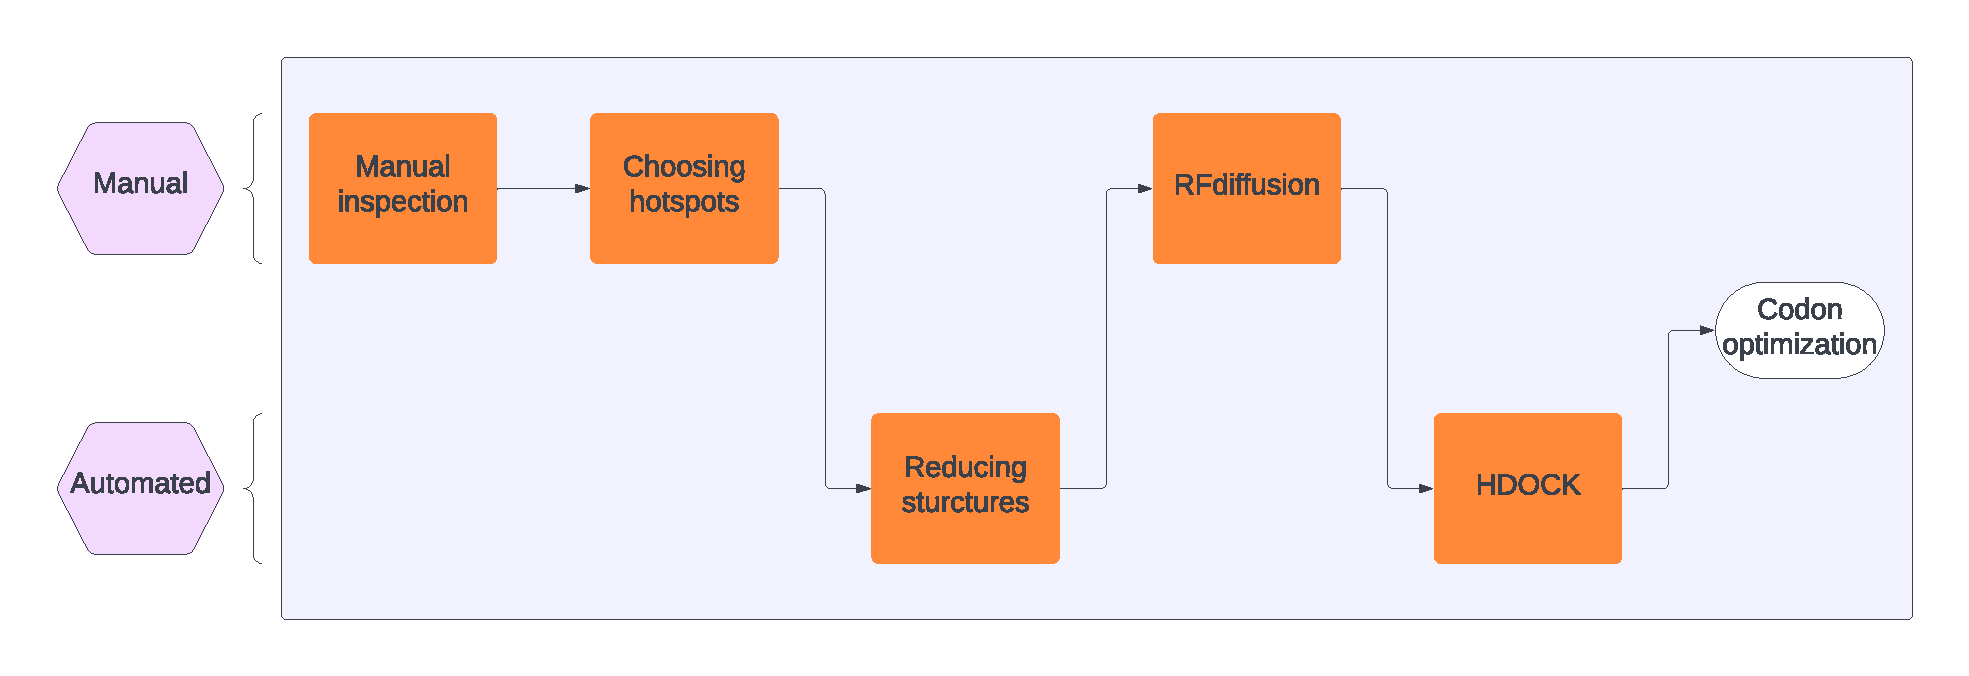
\includegraphics[width=\textwidth]{Supplementary Data/Figures/iGEM_project_general_organization_graph.pdf}
    \caption{General organization graph of the iGEM project.}
    \label{fig:organization_graph}
\end{figure}

\subsection{Target Protein Inspection and Hotspot Selection}

Commencing with the delineation of a hotspot, we define it as a specific residue (amino acid) on the target protein that we aim for the designed binders to effectively bind to. Despite the potential ambiguity of this term, our adoption of RFdiffusion's terminology guides our terminology usage.

Our strategy for selecting potential binding sites involved manual inspection to identify potential hotspots based on specific rules of thumb. We developed these rules of thumb through a combination of manual exploration and adjustments based on RFdiffusion guidance \cite{rfdiffusion_github} and previous studies in this field \cite{chen2013protein}.

Alexis Courbet, a former member of the Baker lab, significantly contributed to shaping our guiding principles for binder design. Leveraging his expertise, we established a set of criteria to guide our manual inspection process, focusing on identifying residues that align with the following:

\begin{itemize}
\item Target regions exhibiting high solvent accessibility.
\item Regions characterized by noticeable hydrophobic patches.
\item Grooves within the target structure.
\end{itemize}


Following the established criteria, we opted for Human Papillomavirus (HPV) as one of our targets due to its nature as a naked virus (non-enveloped) \cite{morshed2014human}. At the initial stages of our exploration of RFdiffusion, the potential interference of glycoproteins with our study was uncertain. To address safety concerns, our strategy involved expressing the proteins in an alternative vector rather than utilizing the actual virus.

We also decided to use Bacteriophage T4 motivated by its availability in our laboratory and the associated safety considerations. Unlike HPV, using the virus in its native form was feasible and, with HPV proteins, presented a robust proof of concept for our study.

To identify hotspots, we employed ChimeraX functionalities such as "hydrophobic" and "electrostatic" to produce an informative depiction of protein surfaces. Figure \ref{fig:protein_inspection_results} illustrates the "hydrophobic" surface of the T4 bacteriophage capsid (Protein Data Bank id: 7vs5). The selected residues (hm19, hm22, hk48, hk49, and fh281) are located within a hydrophobic groove exposed to the solvent, aligning with our design rules.

\begin{figure}[ht]
\centering
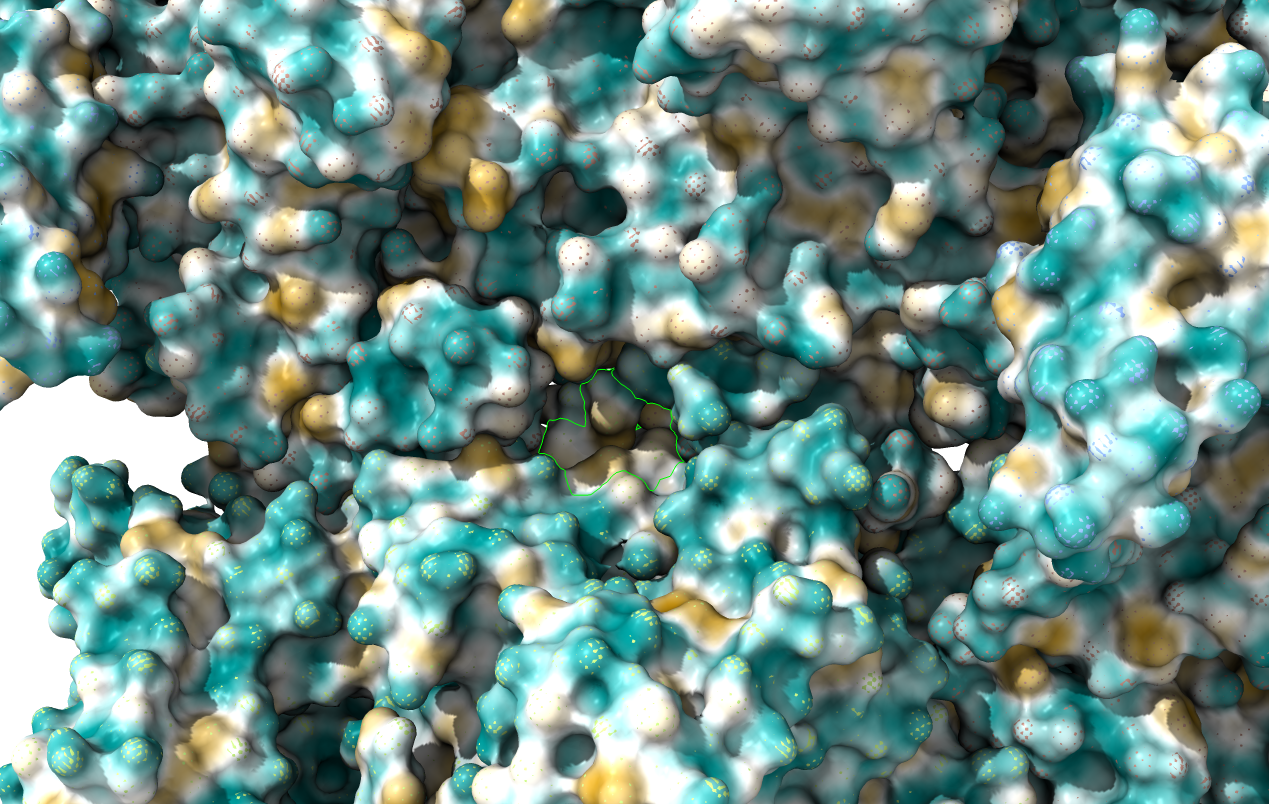
\includegraphics[width=\textwidth]{Supplementary Data/Figures/hydrophobic_view.png}
\caption{Hydrophobic surface of the T4 bacteriophage capsid, generated using ChimeraX. The hydrophobic surface is colored in yellow, while the hydrophilic surface is colored in blue. The selected residues are where we successfully designed two binders.}
\label{fig:protein_inspection_results}
\end{figure}


\subsection{Running RFdiffusion}

To reduce the target protein size, I developed a simple Python script, using the Biopython library \cite{biopython}. The script takes as input a PDB file (or id), a list of hotspots and a radius (in Angstroms). It then outputs a new PDB file containing only the residues within the specified radius of the hotspots. The script is available on the project's GitHub repository (\url{https://github.com/Tony-Makdissy/iGEM_2023}). We wanted to automate this step, in order to minimize the manual steps and the potential errors and biases introduced.

These reduced structures are then manually used as input for RFdiffusion. To comply with legal restrictions, local code execution or connecting a local session to Google Colab is prohibited, as outlined in the \href{https://research.google.com/colaboratory/faq.html#disallowed-activities}{Google Colab disallowed activities}. Therefore, the results of the structure-reducing scripts were manually uploaded to the Google Colab Virtual Machine. Thankfully this step would not produce human biases, but it caused a significant delay in the process.

\subsection{HDOCK: an orthogonal validation approach}

After completing the previous steps, the number of generated sequences reached the order of thousands. However, the practical constraints of our team's budget made it unfeasible to test all these sequences experimentally. To prioritize potential designs and narrow down the candidates for experimental validation, we sought an orthogonal approach for assessment.

Through extensive research, we chose to employ HDOCK, an \emph{in-silico} binding tool \cite{yan2017hdock} known for its consistent performance in the CASP-CAPRI \cite{casp-capri} competition over the years. HDOCK utilizes a Fast-Fourier-Transformation-based docking algorithm, making it a fast rigid body docking tool. Additionally, HDOCK can be used locally, so I developed a Python script to parallelize the process and get all the needed statistics. The script utilizes the "multiprocessing" Python built-in module \cite{python_multiprocessing}.

By the end of this step, only the sequences deemed most likely to exhibit binding were retained for further experimental validation.


\section{Results}

\subsection{RFdiffusion Results}

After manually inspecting four proteins:

\begin{itemize}
    \item HPV major capsid protein (PDB ID: 7kzf)
    \item Bacteriophage T4 capsid (PDB ID: 7vs5)
    \item Bacteriophage T4 Long-Tail (PDB ID: 2xgf)
    \item GFP protein (PDB ID: 5b61)
\end{itemize}

I selected approximately 50 different sets of hotspots, each containing 2 to 6 hotspots, termed as a "run." Refer to the Supplementary Data for the complete table of manual hotspot choices can be found in the folder "Supplementary Data" under the name "Manual choices for hotsopts.csv"

In addition to specifying parameters such as hotspots and the number of sequences, I also uploaded the reduced structures to the Google Colab Virtual Machine (Figure \ref{fig:comparison}).

\begin{figure}[ht]
    \centering
    \begin{subfigure}[b]{0.45\textwidth}
        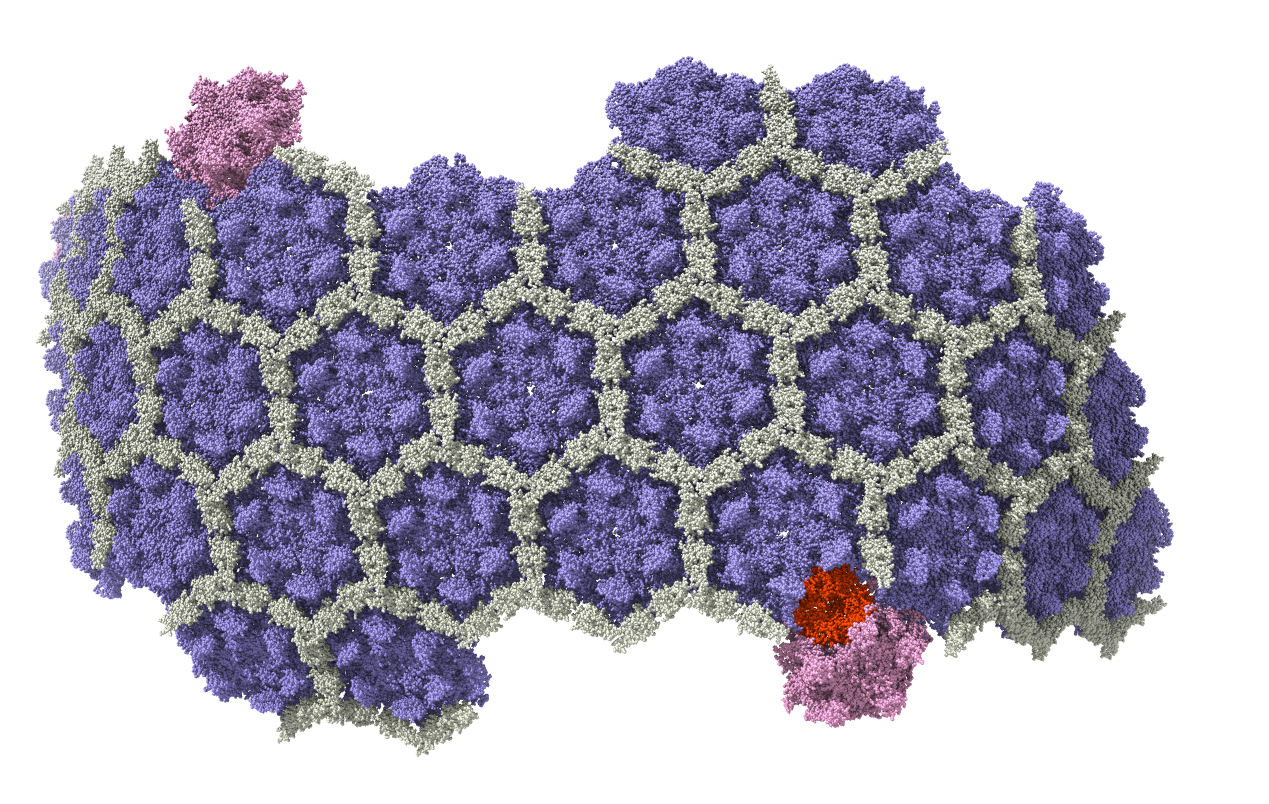
\includegraphics[width=\textwidth]{Supplementary Data/Figures/Full_image.png}
        \caption{Original structure image.}
        \label{fig:full_image}
    \end{subfigure}
    \hfill
    \begin{subfigure}[b]{0.45\textwidth}
        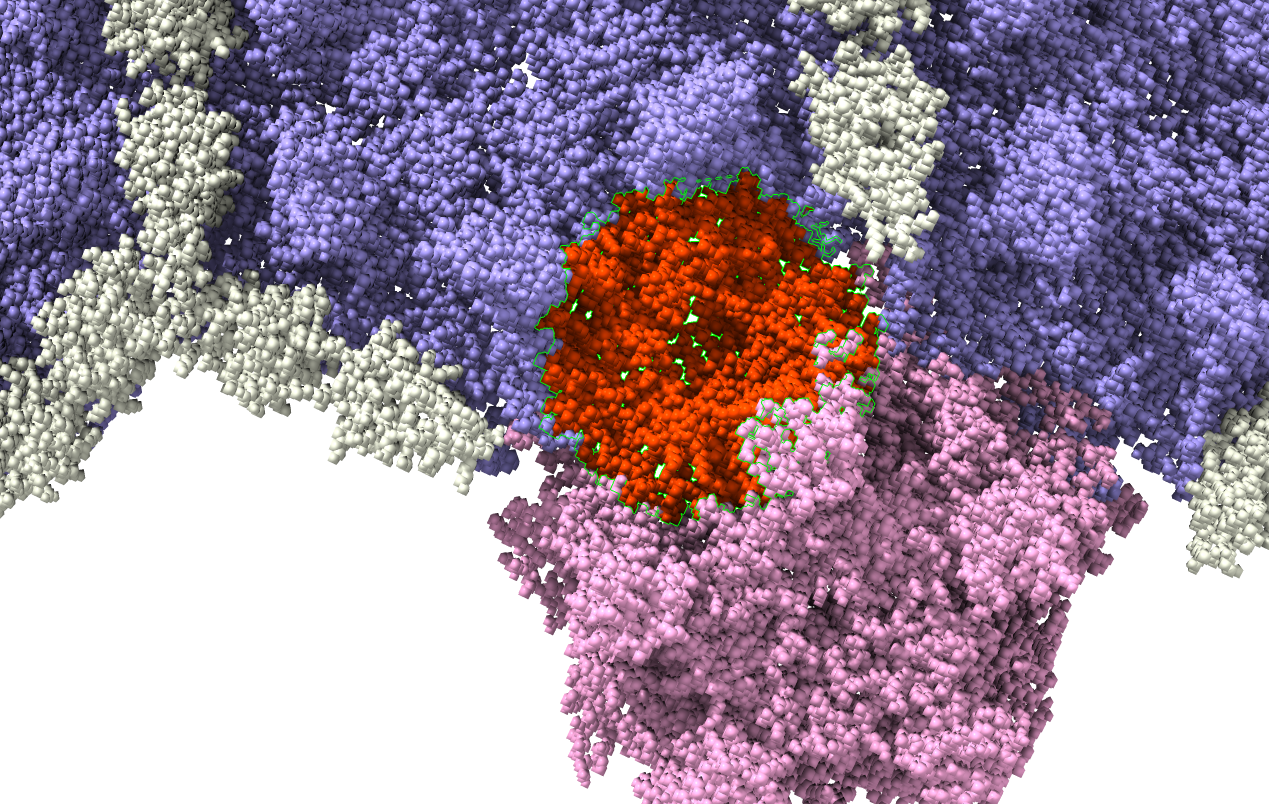
\includegraphics[width=\textwidth]{Supplementary Data/Figures/zoom_4.png}
        \caption{Structure image zoomed four times.}
        \label{fig:zoom_4}
    \end{subfigure}
    \caption{Comparison of the original image and a zoomed image of the structure. The full structure (PDBID 7vs5) has 102,943 residues, while the reduced structure (in orange) has only 514.}
    \label{fig:comparison}
\end{figure}



Each run can generate $S*Q$ sequences, where $S$ represents the number of structure backbones predicted by the RFdiffusion algorithm in the initial step, and $Q$ is the number of sequences generated per structure backbone using the NPMM step.

By the project's conclusion, around 1500 sequences were generated, posing a challenge for experimental testing. To address this, a filtration step was employed using HDOCK.

\subsection{HDOCK Results}

Following the sequence generation, we faced a substantial pool of thousands of sequences, necessitating a method to streamline experimental validation. An in-silico binding assay was chosen, drawing insights from the CASP-CAPRI competitions, renowned for assessing protein structure predictions.

After scrutinizing top-ranking servers in the CASP-CAPRI competition, HDOCK emerged as our choice, driven by its notable attributes:

\begin{itemize}
    \item \textbf{Efficiency:} HDOCK utilizes a high-speed rigid-body docking algorithm grounded in Fast Fourier Transform (FFT).
    \item \textbf{Local Executability and Parallelizability:} In contrast to many web-hosted tools, HDOCK can be locally downloaded and executed, with docking processes parallelizable using the multiprocessing Python library.
    \item \textbf{Proven Performance:} HDOCK secured the 1st rank in CASP-CAPRI11 and continued to excel in subsequent competitions.
\end{itemize}

The selection criteria aimed at choosing best-scoring sequences while ensuring representation from various runs (Figure \ref{fig:universal_score}), enhancing the comprehensiveness of subsequent experimental validation.

One limitation of HDOCK is its lack of experimentally calibrated scores. Scores are not comparable between different target proteins, leading us to compare scores only within the same target. The scores themselves lack a universally meaningful interpretation.


\subsection{Experimental Validation through Pull-Down Assays}

To confirm binding capabilities, pull-down assays were performed on 60 generated sequences. Three showed positive binding to T4 bacteriophage (Figure \ref{fig:universal_score}), validating the computational design (see Table \ref{tab:sequences}). 

\begin{figure}[ht]
    \centering
    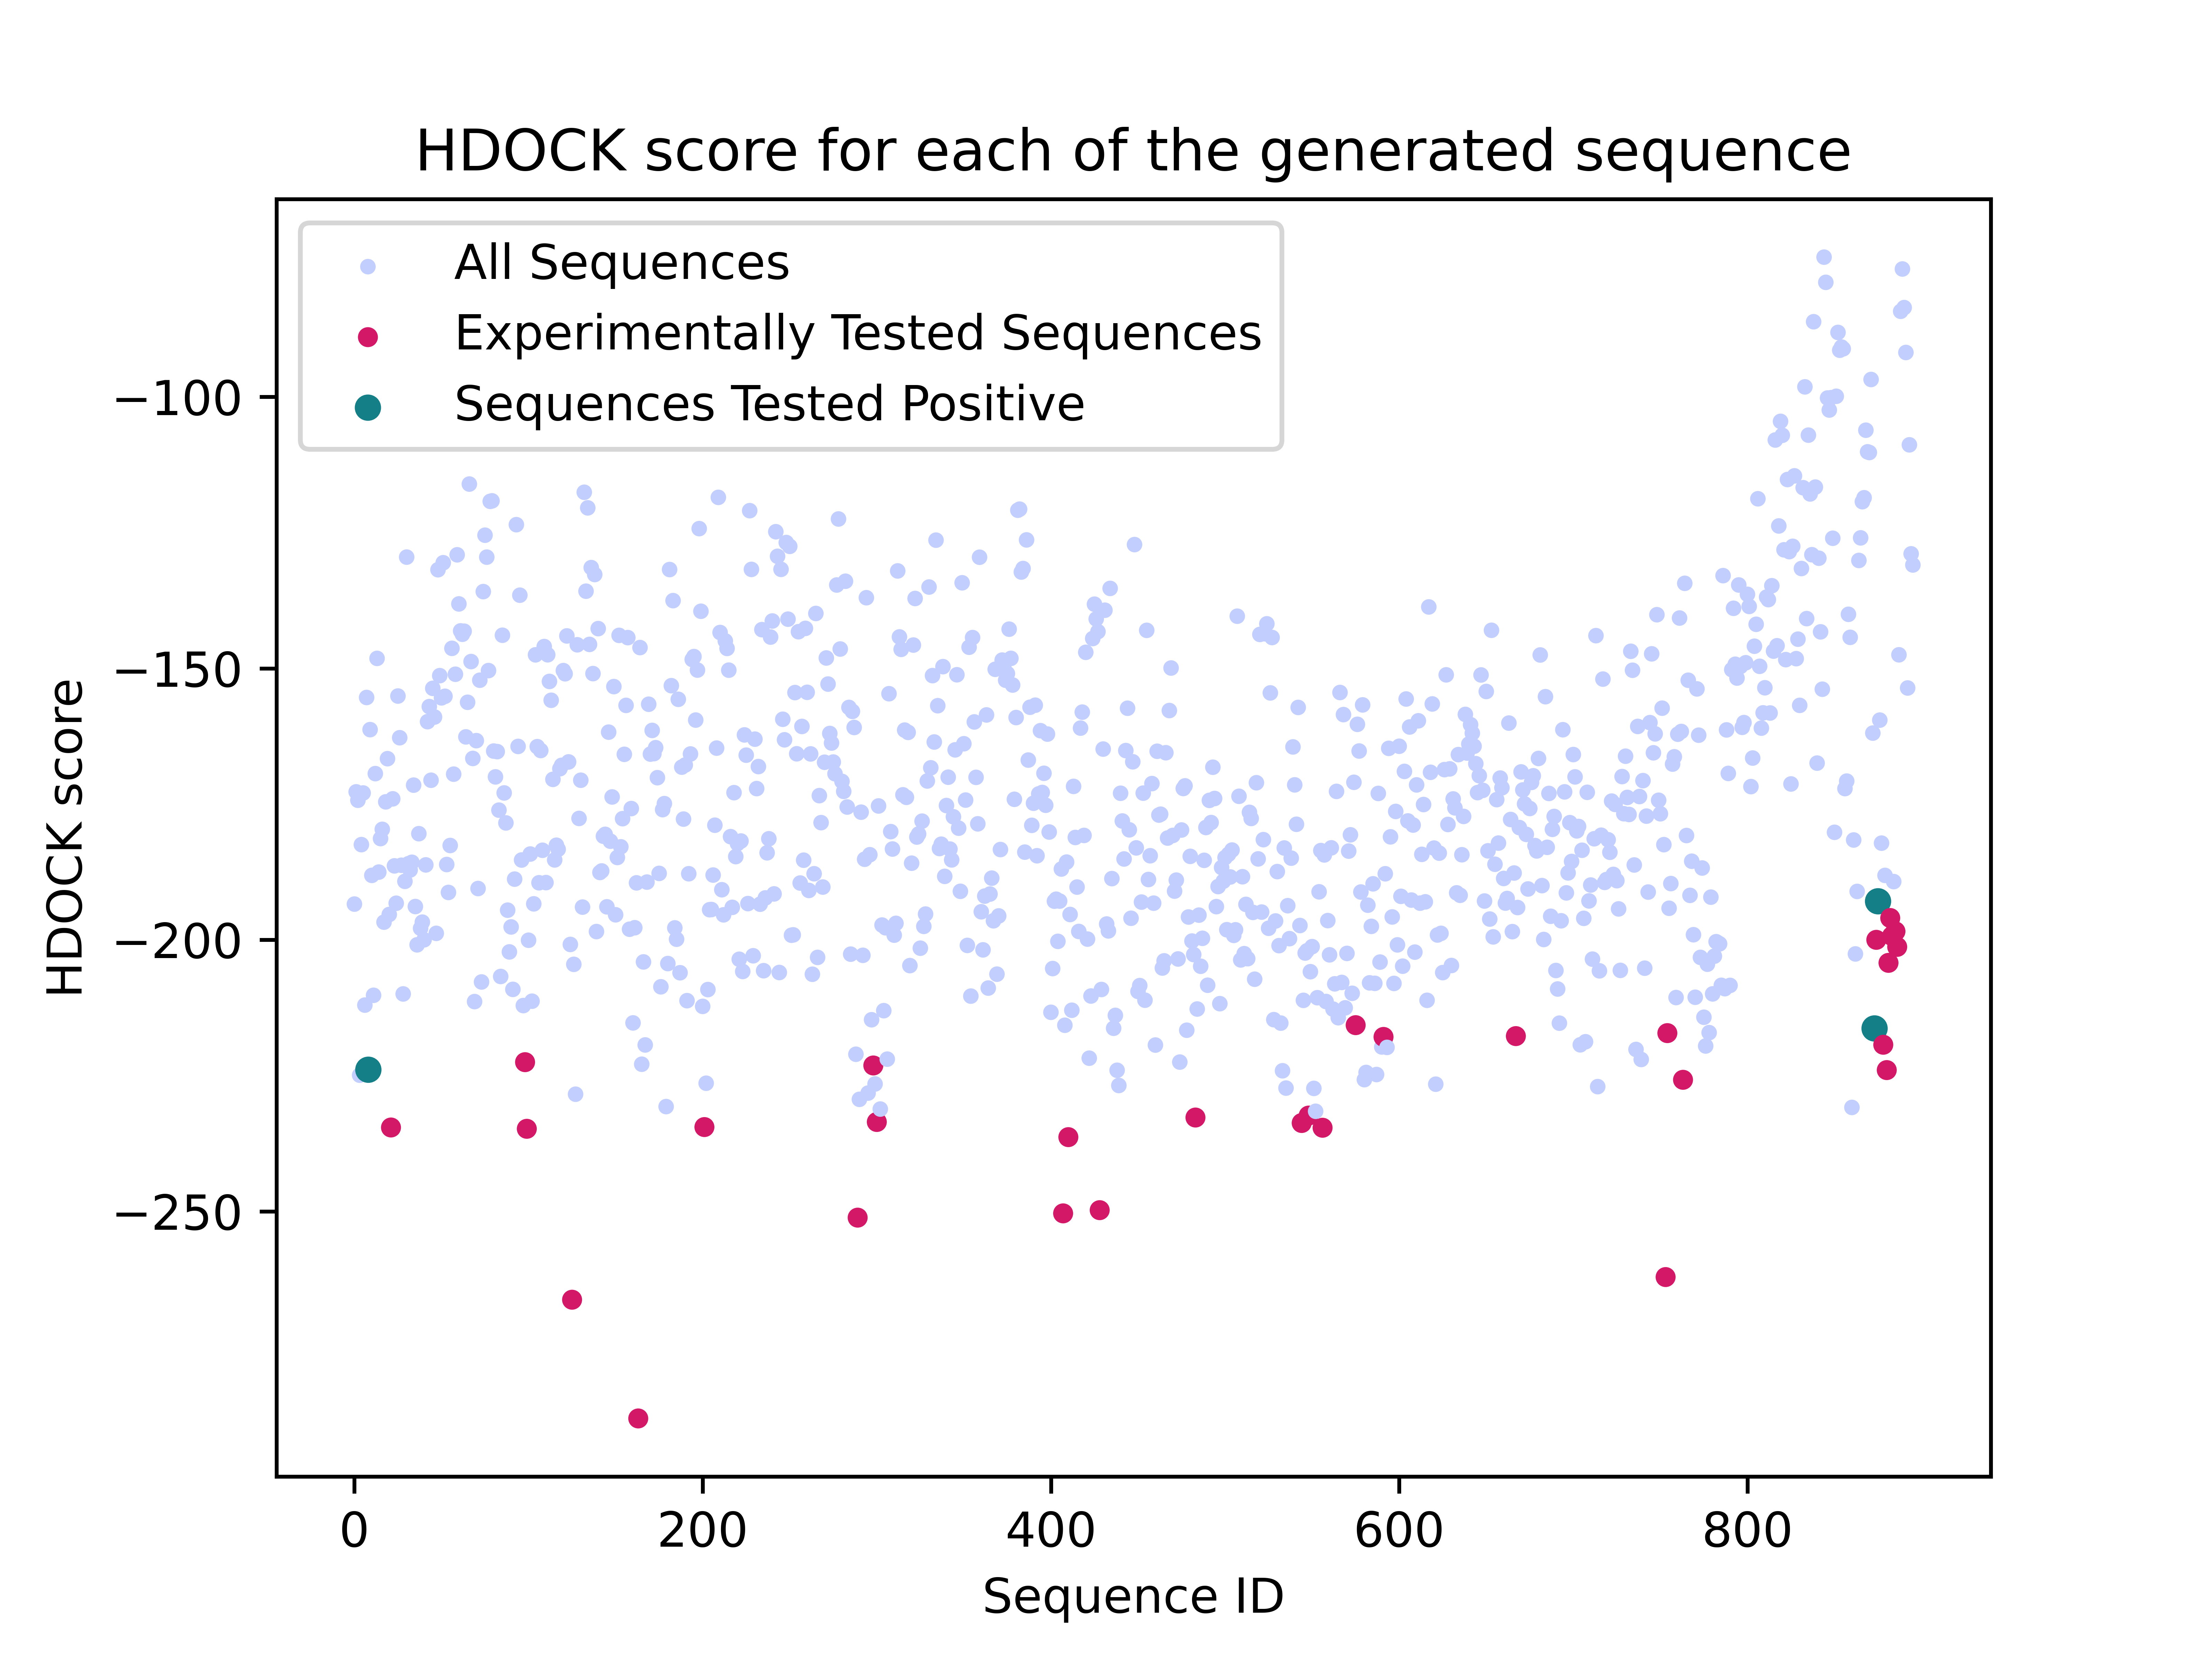
\includegraphics[width=0.9\textwidth]{Supplementary Data/Figures/universal_score_against_Sequence_Global_ID.png}
    \caption{Universal scores against Sequence ID (as used in our tables). Red dots represent all tested sequences, while green dots highlight the three sequences exhibiting positive binding to T4 bacteriophage.}
    \label{fig:universal_score}
\end{figure}

For infectivity assessment, a pull-down phage retention assay was adapted. His-tagged proteins were incubated with T4 phage, and fractions were collected through an affinity purification column. Phage concentrations were quantified using a plaque assay. This setup, inspired by existing literature, provides insights into the designed protein's impact on viral infectivity.

I did not contribute to this step; credit goes to my friends Avi, Mostafa, and Louis for handling wet lab activities.

\subsection{Further Analysis}

After validating three sequences, a BLAST search yielded no matches with known proteins under default parameters. This supports RFdiffusion's potential for generating novel sequences.

A video demonstrating a hypothetical binding scenario is available in the "Supplementary Data" folder as "Binding\_video.mp4." The binder, designed based on an AlphaFold2 prediction, is expected to bind to the area shown in Figure \ref{fig:protein_inspection_results} (T4 bacteriophage capsid structure from PDB ID 7vs5). The code used to generate the video is available on the following GitHub repository: \url{https://github.com/Tony-Makdissy/iGEM_final_presentation}


\subsection{iGEM Results}

Despite achieving promising results in our project, we faced a setback as we failed to complete the required paperwork within the specified time, ultimately leading to our disqualification \frownie{}. 

\section{Discussion}

Our study successfully demonstrates the design and experimental testing of several proteins that do not exist in nature within an unusually short timeframe. This achievement is a testament to the potential of our approach in expanding the repertoire of available proteins.

Despite the success, challenges remain in fully automating the process. Computational resources, in theory, could support automation; however, manual inspection remains a necessity. A profound understanding of differential geometry is crucial for defining hydrophobic grooves and other geometric features. This manual intervention represents a current bottleneck in the workflow.

Our work lays a robust foundation for further research in this field. While the number of positively binding proteins is promising, achieving statistical significance requires more comprehensive studies. The sequences demand further investigation into their true structure and binding kinetics, as these structures were only assayed for binding. Additionally, optimizing the code remains an avenue for future improvements.

Moreover, it is crucial to acknowledge that the scope of our work extends beyond Lubretict. The protein generation and \emph{in-silico} binding assays are blind to the overall scope. This pipeline holds potential beyond our current application and can be adapted for the generation of binders in diverse contexts.

\emph{De novo} proteins require extra caution in their potential applications, especially regarding their interactions with living organisms, such as humans. The implications of introducing these novel sequences into biological systems necessitate comprehensive studies to understand their safety and efficacy. Additionally, even though a cell can produce a given sequence, the efficiency of production and the ability to fine-tune these sequences remain unknown. Ongoing studies in this field aim to shed light on these aspects, contributing to a more comprehensive understanding of the practical implications of de novo protein design.

\section{Conclusion}

In conclusion, our research not only marks a significant step forward in protein design and testing but also outlines a versatile pipeline with applications that stretch beyond the immediate scope. Collaborative opportunities, practical implications, and the potential for future advancements further underscore the significance of our work in the broader scientific landscape.


\section*{Acknowledgments}

We extend our gratitude to Minc's Lab, Institute Jacques Monod, and IFB - Institut Français de Bioinformatique for server access crucial to our computational tasks.

Special thanks to Alex and Sergey for invaluable assistance in protocol design, and to the Life Sciences Institute (LPI) team for continuous support, and fostering innovation.


\section*{Data Availability}

As the team is planning to publish the results of this project in a peer-reviewed journal, the data is not available yet. However, the code is available on GitHub (\url{https://github.com/Tony-Makdissy/iGEM_2023}). Along with the successfully validated sequences (Table \ref{tab:sequences}) and the list of run's parameters (see Supplementary Data).

A full list of all the runs' sequences with their corresponding statistics and experimental data will be available after the publication of the paper.

For this report, you can access the \LaTeX\ code used to create it following the link \url{https://github.com/Tony-Makdissy/internship_report_2024_autumn} which contains all the code and data used to create this report.

Supplementary Data will be provided as a separate file along with the report and can be accessed on the GitHub Repository.

% References
\printbibliography

\newpage

\section*{Annexes}

\subsection*{Table of free and open-source tools used in the project}


\begin{table}[ht]
    \centering
    \caption{List of Open-Source Tools Used in the Project}
    \label{tab:tools}
    \begin{tabular}{p{2.5cm}|p{14cm}}
    \toprule
    Tool name & Links \\
    \midrule
    RFDiffusion & GitHub Repository: \\
     & \url{https://github.com/RosettaCommons/RFdiffusion} \\
     & Google Colab Notebook: \\
     & \url{https://colab.research.google.com/github/sokrypton/ColabDesign/blob/main/rf/examples/diffusion.ipynb} \\
    HDOCK & Website: \url{http://hdock.phys.hust.edu.cn/} \\
    AlphaFold2 & GitHub Repository: \\
     & \url{https://github.com/google-deepmind/alphafold} \\
     & Google Colab Notebook: \\
     & \url{https://colab.research.google.com/github/deepmind/alphafold/blob/main/notebooks/AlphaFold.ipynb} \\
    RosettaSurf & GitHub Repository: \\
     & \url{https://github.com/LPDI-EPFL/RosettaSurf} \\
    ESMFold & GitHub Repository: \\
     & \url{https://github.com/facebookresearch/esm} \\
     & Google Colab Notebook: \\
     & \url{https://colab.research.google.com/github/sokrypton/ColabFold/blob/main/ESMFold.ipynb} \\
    RoseTTAFold & GitHub Repository: \\
     & \url{https://github.com/RosettaCommons/RoseTTAFold} \\
     & Google Colab Notebook: \\
     & \url{https://colab.research.google.com/github/sokrypton/ColabFold/blob/main/RoseTTAFold.ipynb} \\
    ChimeraX & GitHub Repository: \\
    & \url{https://github.com/RBVI/ChimeraX} \\
    & Website: \\
    & \url{https://www.rbvi.ucsf.edu/chimerax/} \\
    \bottomrule
    \end{tabular}
\end{table}

\newpage

\subsection*{Table of experimentally validated sequences}

\begin{table}[ht]
    \centering
    \caption{Experimentally validated sequences and their corresponding target Protein Data Bank (PDB) IDs}
    \begin{tabular}{|c|p{10cm}|}
        \hline
        \textbf{Target PDBID} & \textbf{Sequence} \\
        \hline
        2xgf & \seqsplit{DLEALRAAIRAEADARAAAFVARPPLTPAERAALAARLRARLAGRPDADARVAALRRLSPVAQLAERYRREAAERAAEVAALIPEGPEVAAYILQRANDAAATLRAAA} \\
        \hline
        7vs5 & \seqsplit{MSNTLEQKIISARAVDADALLARVLARLDALAAEDPSHAAELAALRATIAEAQALAATAAPIPLRDLAIALRERARALRAKDSAKNRRLVRLTDEAADLVRVLIAQALA} \\
        \hline
        7vs5 & \seqsplit{MSSTLEQKIISSKAVDVEELLKRVLERLEELEKKDPKHKEKLEELRKKIEKALELAKTSTYVPLLDLAIELENEAQKLRGENAKENSELVRLTDEAADLVRAMISKALQ} \\
        \hline
    \end{tabular}
    \label{tab:sequences}
\end{table}

\end{document}  